\documentclass[10pt]{beamer}

\usetheme[background=dark, numbering=fraction]{metropolis}
\usepackage{appendixnumberbeamer}
\usepackage{color, xcolor}
\usepackage{dsfont}
\definecolor{mydarkblue}{rgb}{0,0.08,0.45}


\usepackage{booktabs}
\usepackage[scale=2]{ccicons}


\usepackage{adjustbox} 
\usepackage{pgfplots}
\usepgfplotslibrary{dateplot}
\usepackage{fourier-orns}
\usepackage{xspace}


\newcommand{\themename}{\textbf{\textsc{metropolis}}\xspace}
\DeclareMathOperator*{\argmin}{arg\,min}
\DeclareMathOperator*{\minimize}{minimize}
\DeclareMathOperator*{\maximize}{maximize}

\makeatletter
\renewcommand{\metropolis@colors@dark}{%
  \setbeamercolor{normal text}{%
    fg=black!2,
    bg=mDarkTeal
  }%
  \usebeamercolor[fg]{normal text}%
}
\renewcommand{\metropolis@colors@light}{%
  \setbeamercolor{normal text}{%
    fg=mDarkTeal,
    bg=black!2
  }%
  \usebeamercolor[fg]{normal text}%
}
\makeatother

\title{Parallel Optimization and Machine Learning}
\date{\today}
\author{Fabian Pedregosa}
\institute{UC Berkeley}
%\titlegraphic{\hfill\includegraphics[height=1.5cm]{figures/UCBerkeley_wordmark_blue.eps}}

\begin{document}

\maketitle

\metroset{background=light} % change background theme according to manual
{
\usebackgroundtemplate{%
\begin{picture}(40,260)
  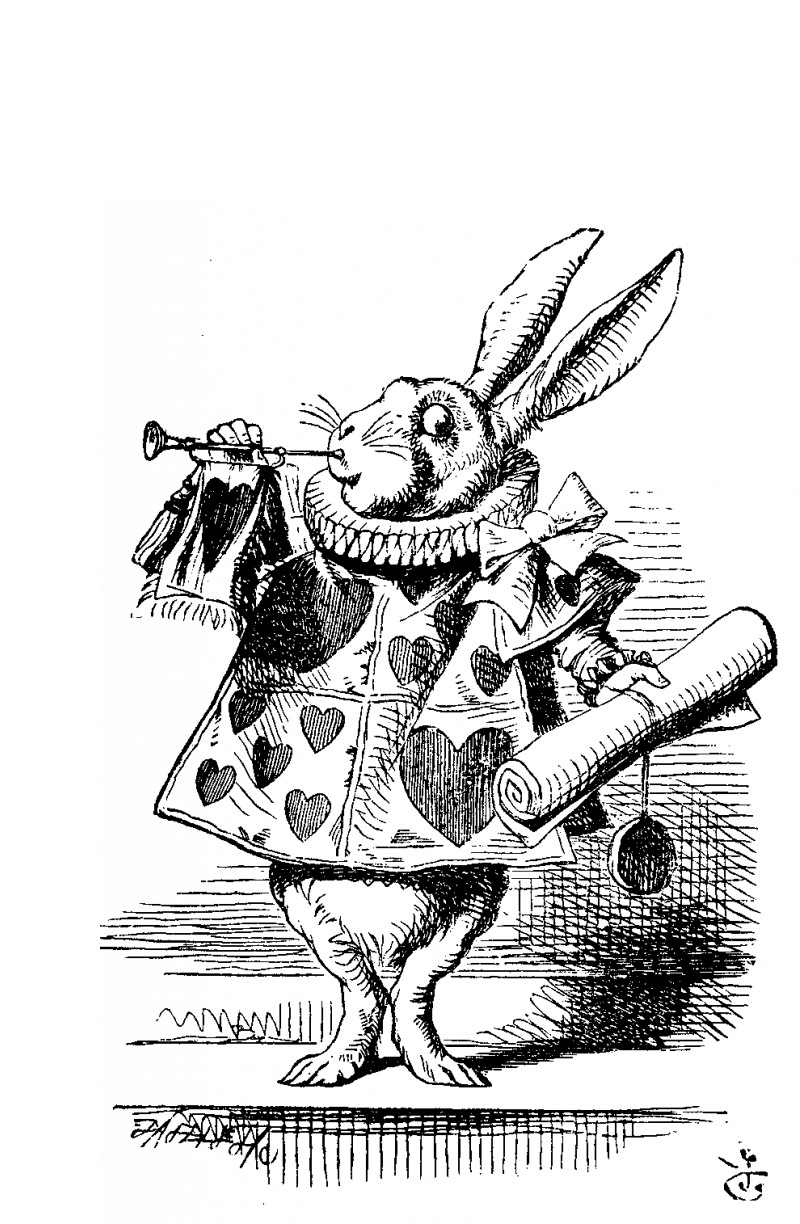
\includegraphics[height=0.9\paperheight]{img/white-rabbit}
  \end{picture}
  }
\begin{frame}{About me}
\begin{column}{0.5\textwidth}  %%<--- here
\end{column}
\begin{column}{0.5\textwidth}  %%<--- here
\end{column}
\end{frame}
}

\metroset{background=dark} % change background theme according to manual
\begin{frame}{Today's lecture}
  \begin{itemize}
    \item Student presentation
    \item Unsupervised learning: PCA and K-means.
    \item Hands on applications: 
    \begin{itemize}
    \item Faces ``basis'' or eigenfaces.
    \item Stock market analysis using clustering.
    \end{itemize}
    \item Next lecture: deep learning (machine learning competition)
  \end{itemize}
\end{frame}
% 
% \begin{frame}{Logistic regression}
%     Pillar of supervised learning. One of the most common methods
% 
%     Two motivations
% 	\begin{itemize}
% 		\item As a probabilistic model.
% 		\item Mathematical optimization.
% 	\end{itemize}
% \end{frame}
% 
% 
% 
% \section{Probabilistic model}
% 
% \begin{frame}[fragile]{Probabilistic view}
% \begin{center}
% {\bfseries Motivation}: classification problem with two classes.
% 
% \vspace{1em}Classes = ``-1'' and ``1'', which represent outcomes such as pass/fail, win/lose, alive/dead or healthy/sick, etc.
% 
% \vspace{1em}
% \danger\alert{Despite its name, logistic regression is a model for classification and not regression.}
% \end{center}
% \end{frame}
% 
% \begin{frame}[fragile]{Probabilistic view}
% \begin{center}
% {\bfseries Motivation}: Cancer / no cancer as a function of biomarker.
% \includegraphics[width=0.8\linewidth]{figures/logistic_1.pdf}
% 
% \end{center}
% \end{frame}
% 
% \begin{frame}[fragile]{Probabilistic view}
% \begin{center}
% {\bfseries Motivation}: Cancer / no cancer as a function of biomarker.
% \includegraphics[width=0.8\linewidth]{figures/logistic_2.pdf}
% 
% \pause
% \alert{Goal}: Given new data, estimate the probability of having cancer \hfill \\
% $\iff$ estimate {$P(Y=1|X)$}
% \end{center}
% \end{frame}
% 
% 
% \begin{frame}[fragile]{Probabilistic view}
% 
% 
% \begin{columns}[t]
% \begin{column}{.5\textwidth}
% One popular model for  {$P(Y=1|X)$} is the logistic model,
% 
% \begin{align*}
% &P(Y=y_i|X=x_i) = \sigma(y_i(x_i^T \beta_1 + \beta_0))\\
% &\quad \text{with } \sigma(t) = \frac{\exp(t)}{1 + \exp(t)}
% \end{align*}
% 
% \end{column}
% \begin{column}{.5\textwidth}
% \adjincludegraphics[width=0.8\linewidth,valign=t]{figures/sigmoid}\hfill\\
% The logistic function $\sigma(t)$
% \end{column}
% \end{columns}
% 
% \vspace{1em}
% In the 1D case we have 2 degrees of freedom, $\beta_1, \beta_0$ that control the slope and intercept of the approximation.
% \pause
% In the $p$-dimensional case, we have $p+1$-degrees of freedom, as $\beta_1 \in \mathbb{R}^p, \beta_i \in \mathbb{R}$
% \end{frame}
% 
% 
% \begin{frame}[fragile]{Inference}
% The coefficients $\beta_1, \beta_0$ can be estimated as the ones that maximize the likelihood given the current data $\{(y_1, x_1), \ldots, (x_n, y_n)\}$.
% $$
% \maximize_{\beta_1, \beta_0}\,\ell(\beta_1, \beta_0) = \prod^n_{i=1} P(Y=y_i|X=x_i)
% $$
% 
% \pause
% Although for numerical reasons we rather minimize the minus log-likelihood
% \begin{align}
% \minimize_{\beta_1, \beta_0}\,-\log(\ell(\beta_1, \beta_0)) &= \sum^n_{i=1} -\log(P(Y=y_i|X=x_i))\\
% &= \sum^n_{i=1} \log(1 + \exp(-y_i ( x_i^T \beta_1 + \beta_0)))\label{eq:log_loss}
% \end{align}
% \end{frame}
% 
% \section{Regularization}
% 
% \begin{frame}
% In the $p$-dimensional setting. 
% \end{frame}
% 
% \begin{frame}[fragile]{Generalization}
% This approach can be naturally generalized to $K$ classes.
% \begin{align}
% \Pr(Y_i=1) &= \frac{e^{\boldsymbol\beta_1 \cdot \mathbf{X}_i}}{1 + \sum_{k=1}^{K-1} e^{\boldsymbol\beta_k \cdot \mathbf{X}_i}} \nonumber \\
% \Pr(Y_i=2) &= \frac{e^{\boldsymbol\beta_2 \cdot \mathbf{X}_i}}{1 + \sum_{k=1}^{K-1} e^{\boldsymbol\beta_k \cdot \mathbf{X}_i}} \\
% \cdots & \cdots \\
% \Pr(Y_i=K-1) &= \frac{e^{\boldsymbol\beta_{K-1} \cdot \mathbf{X}_i}}{1 + \sum_{k=1}^{K-1} e^{\boldsymbol\beta_k \cdot \mathbf{X}_i}}
% \end{align}
% \end{frame}
% 
% 
% \begin{frame}[fragile]{Application}
% Lets use this to predict the future!
% 
% \pause
% Use the data from the religion dataset to predict how religious beliefs will evolve after 2017
% 
% \includegraphics[width=0.5\linewidth]{figures/religion.png}
% 
% \pause
% Suggestion: use scikit-learn's LogisticRegression class with {multi\_class='multinomial'}. Use as features the year and cohort. The model can predict probabilities with method predict\_proba.
% 
% \end{frame}
% 
% 
% 
% \begin{frame}[fragile]{Application}
% 
% 
% To predict, use the same data but with year and cohort shifted accordingly.
% 
% \includegraphics[width=0.5\linewidth]{figures/logistic_future.png}
% 
% 
% 
% \end{frame}
% 
% 
% 
% \nocite{*}
% 
% \begin{frame}[allowframebreaks]{References}
% 
%   \bibliography{demo}
%   \bibliographystyle{abbrv}
% 
% \end{frame}

\end{document}
